\subsection{Homonukleare Moleküle (Beispiel $H_2$)}
	\begin{figure*} [h]
		\begin{center}
			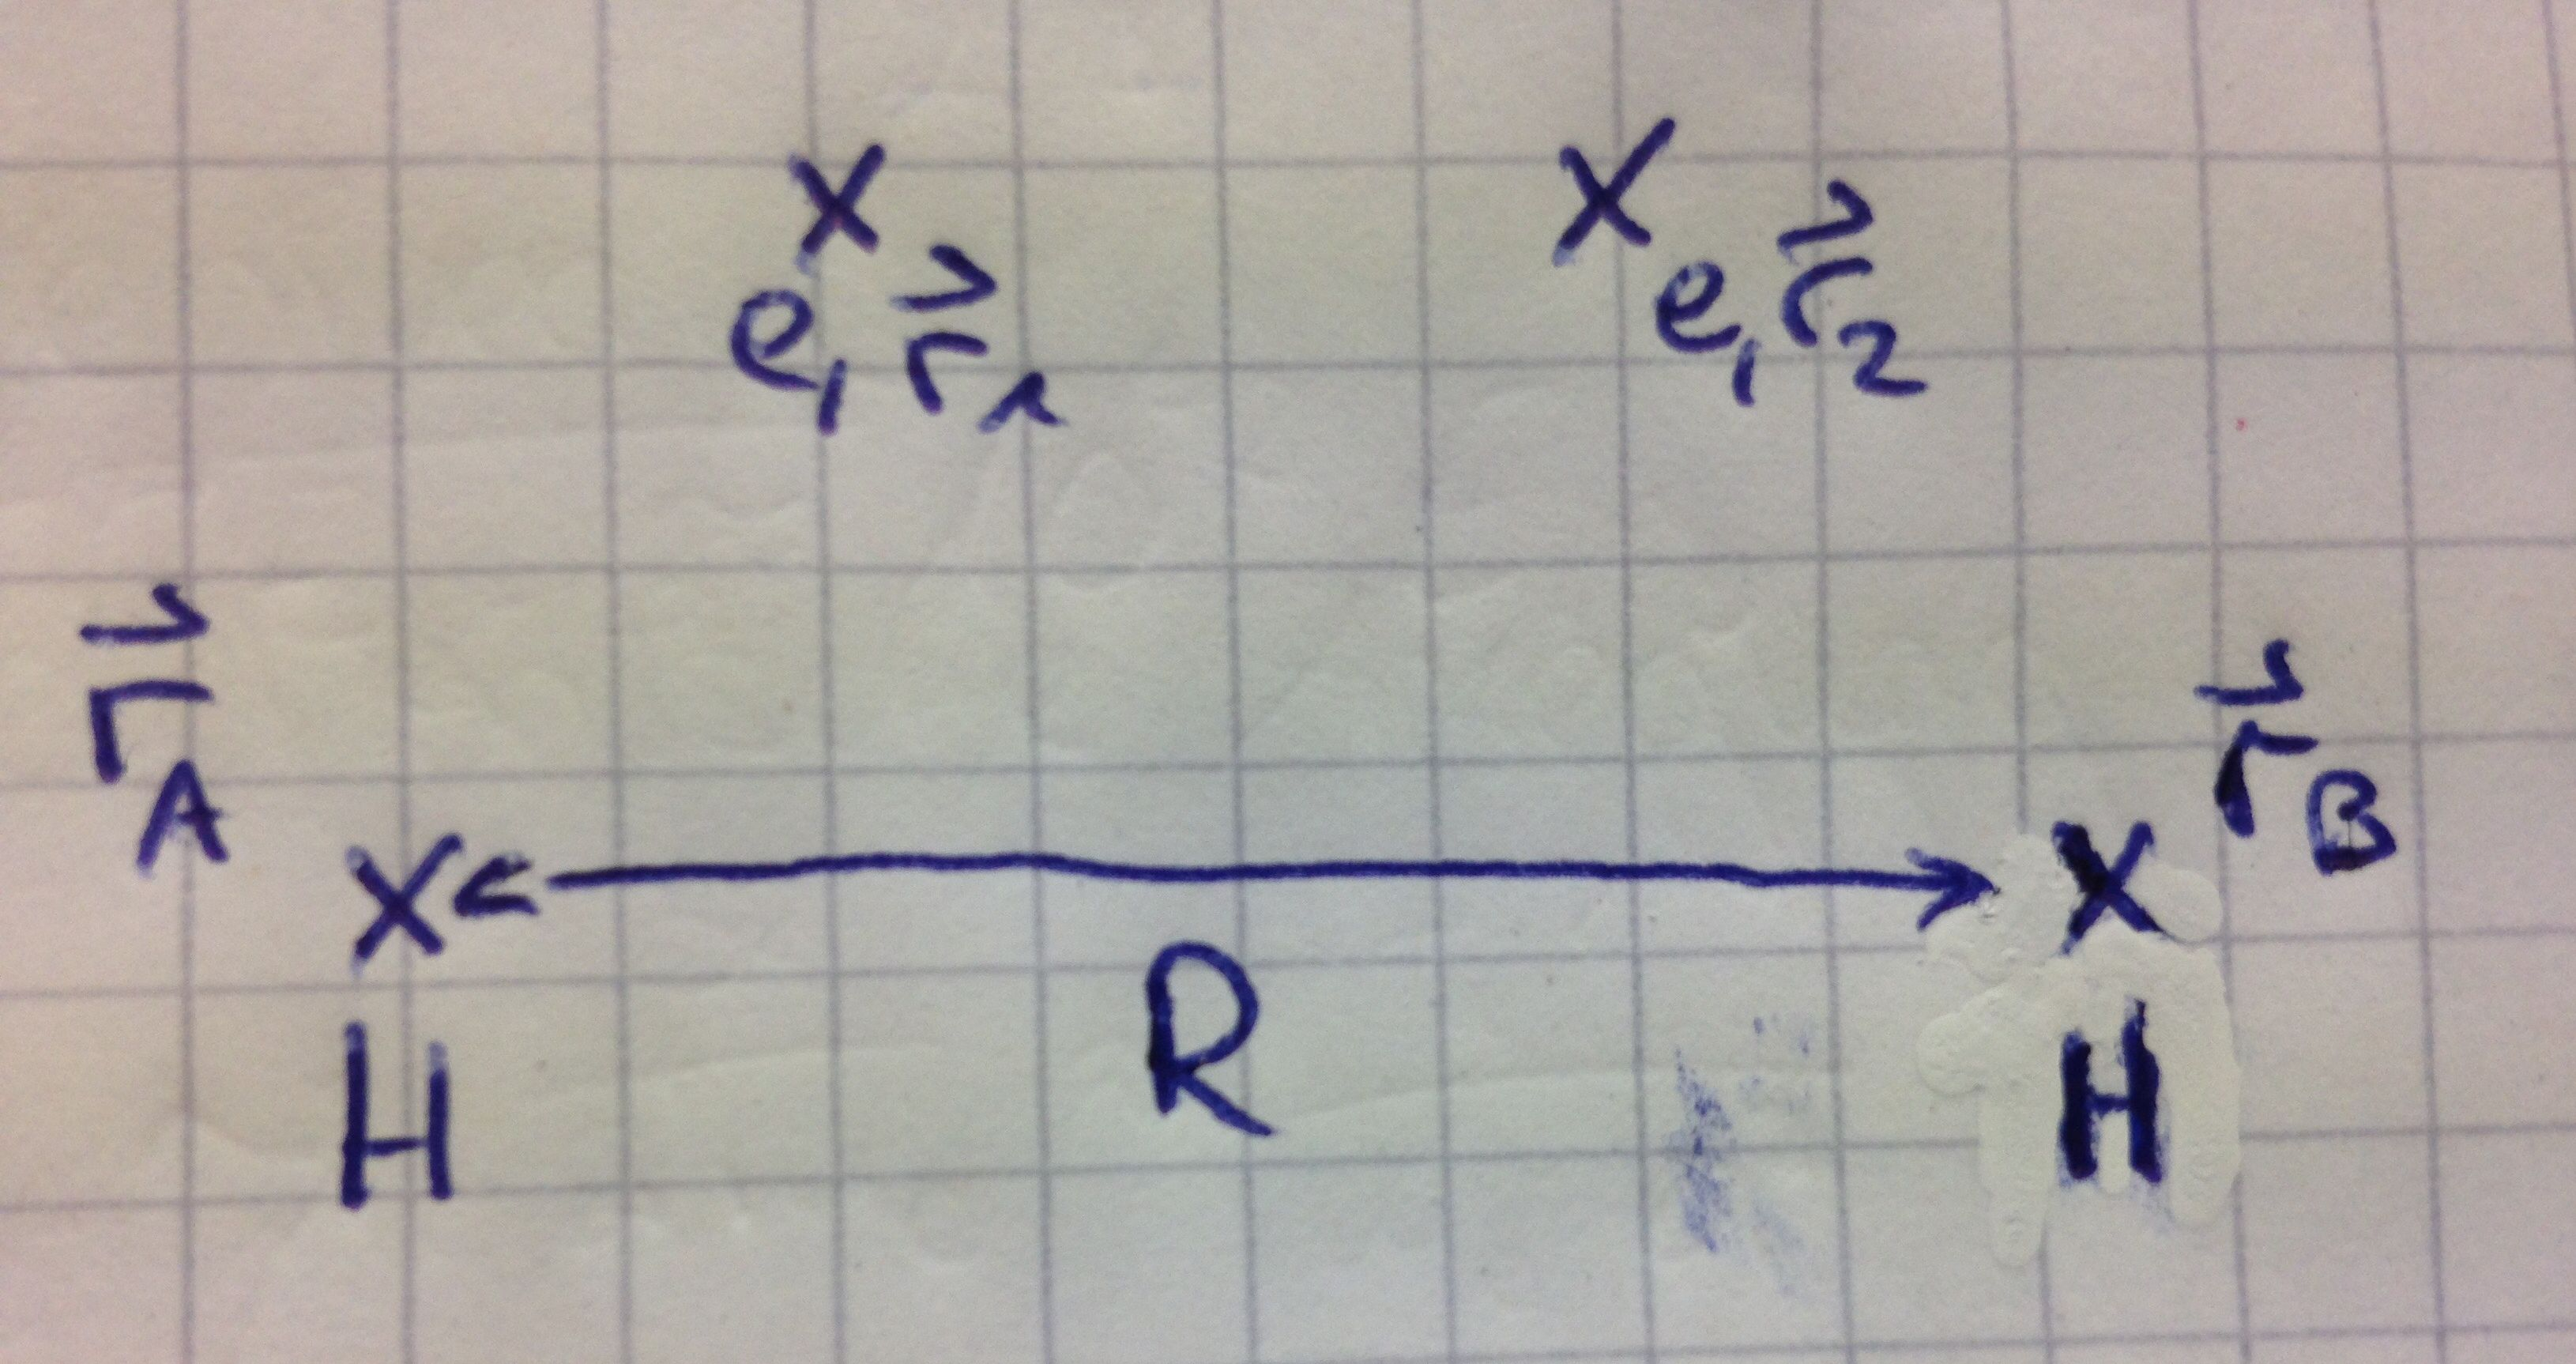
\includegraphics[width=10cm]{Homonukleare_Molekuele1}
		\end{center}
	\end{figure*}
	\begin{align*}
		R = | \vec{r}_A - \vec{r}_B |
	\end{align*}
	\begin{align*}
		R \rightarrow \infty &: \text{Separiert in 2 ``isolierte'' }H \text{-Atome} \\
		R \rightarrow 0 &: He\text{-Wellenfunktion}
	\end{align*}
Rotationssymmetrie gebrochen zu zylindrischer Symmetrie
	\begin{align*}
		C_\infty &\subset \mathscr{O} (3) 
		&\text{Homonuklear } C_{\infty_h} &= C_{\infty_h} \times C_i
	\end{align*}
$C_i$ ist die Parität

$L, J,$etc. keine ``guten'' Quantenzahlen.

Projektionvon $\vec{L}$ auf Molekühlachse $\Lambda$ ist erhalten
	\begin{align*}
		\Lambda &= 0, 1, 2, \ldots ,&
		\Lambda_z &= \pm \Lambda ~(\text{analog zu } m, \text{ aber } m = -\ell, +\ell) \\
		&\left(\sum, \prod, \Delta, \text{etc.}\right)
		& ^{2S + 1}\Lambda &, \text{z.B. } ^3 \prod ~(\text{Spin-Triplet}) 
	\end{align*}
Weitere Symmetrie: Spiegelung an Ebene
	\begin{figure*} [h]
		\begin{center}
			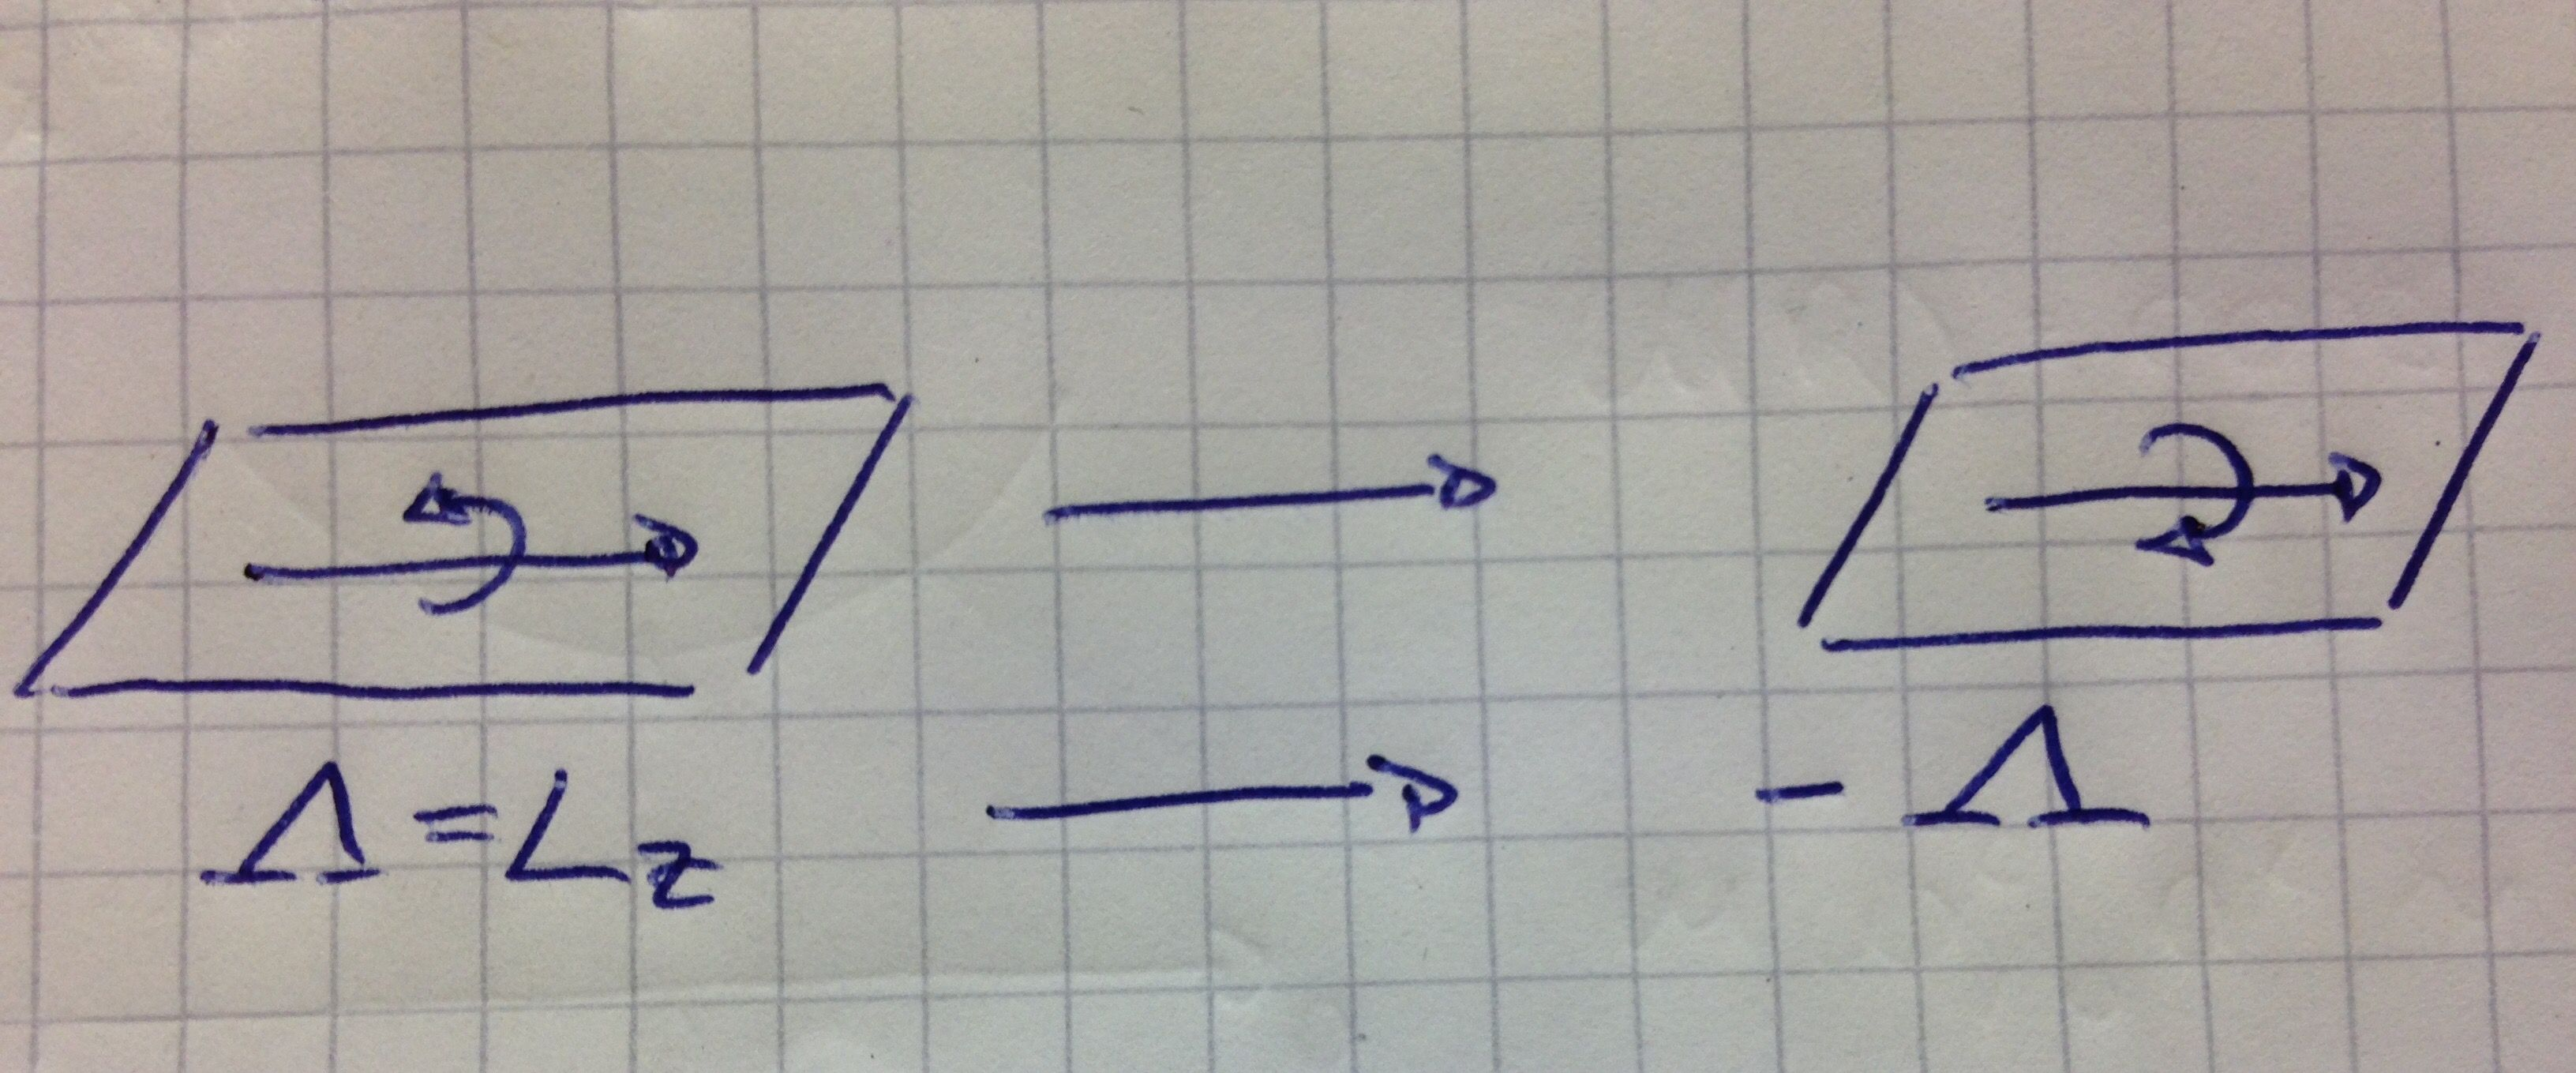
\includegraphics[width=10cm]{Homonukleare_Molekuele2}
		\end{center}
	\end{figure*}
	\begin{align*}
		\Lambda > 0 &: \text{Zustände sind 2-fach entartet. } (\text{analog zu } 2 \ell + 1 \text{ bei Rotationssymmetrie}) \\
		\Lambda = 0 &: \text{Eigenwerte } \sigma_V = + 1, \text{ oder } \sigma_V = -1.\\
		&\curvearrowright {\sum}^+ oder {\sum}^-
	\end{align*}
Homonuklear: Inversion am Mittelpunkt
	
$\Rightarrow$ Parität $\eta = g, u$ 
\\
Molekühlorbits:
	\begin{align*}
		^{2 S + 1}{\sum}_{g, u}^{+ , -} , ^{2 S + 1} {\prod}_{g, u}, ^{2 S + 1}\Delta_{g, u}, \ldots
	\end{align*}
Grundzustand: Bahnwellenfunktion 

hat keine Knotetn $\curvearrowright \eta = g, \sigma_V = +$.
\\
Bahnwellenfunktion ist symmetrisch unter
	\begin{align*}
		\vec{r} \rightarrow - \vec{r} &\Rightarrow \text{ Spinwellenfunktion ist antisymmetrisch}\\
		&\Rightarrow S = 0
	\end{align*}
Wir interessieren uns für 	
	\begin{align*}
		^1{\sum}^+, ^1{\sum}^+_g ~(\text{homonuklear})
	\end{align*}
``Ausnahme'':
	\begin{align*}
		O_2 &: ^3{\sum}^-_g & &\text{hier kommen zeichnungen hin, }\\
		NO &: ^2\prod & &\text{hab aber zu wenig ahnung von Chemielatexzeugsi}
	\end{align*}
	\begin{align*}
		R &\rightarrow 0 : He &\text{Parität } P &\rightarrow \eta = (-)^{S + L}
		&(\vec{r}_i \rightarrow -\vec{r}_i \text{ nicht } \vec{r}_1 \leftrightarrow \vec{r}_2) \\
		\Lambda &= 0 &{\sum}^{(-)^L \cdot \eta} &= {\sum}^{(-)^S}
	\end{align*}
$R \rightarrow 0$ verschiedene $D_{\infty_h}$ Zuständie geben dasselbe $J^{PC}$ (was das auch immer sein möge, ich hab echt keine Ahnung)

	\begin{tabular}{l l}
		He & H$_2$ \\
		$^1S_0$ & $^1{\sum}^+_g$ \\
		$^3S_1$ & $^3{\sum}^-_u$ \\
		$^1P_1$ & $^1{\sum}^+_u, ^1{\prod}_u$\\
		$^3P_{0,1,2}$ & $^3{\sum}^-_g, ^3{\prod}_g$\\
	\end{tabular}
	
Und hier war noch eine skurile Zeichnung, die keiner verstanden hat ;-)

